% ======================================================================
% Submission version (NMI / Nature Computational Science, 2026-08-24).
% Condensed from the frozen full version in ../tex/ with an identical
% logic chain; displaced protocol detail lives in methods.tex.
% ======================================================================
\section{Results}

\subsection{Autonomous discovery of eight laws by proposal, test and refutation}
\label{sec:loop}

Crystal chemistry constrains a structure through a few measurable quantities. A law
worth testing must name one of them in a one-line statement a chemist can read,
calculate and try to disprove: one that experimental structures satisfy but prescribed
perturbations of them violate. Autonomous agents propose such
statements rapidly, but only testing rules out the false explanations for an apparent
success. Our
agents proposed and implemented hypotheses and selected thresholds on a discovery split, then
designed counterexamples and attempted refutation with held-out data and physical
checks (Fig.~\ref{fig:loop}a). Refuted claims remained in the record as diagnostics for
the next cycle, so these cycles formed a sequence of falsifiable experiments (Supplementary
Figs.~\ref{si-sifig:ledger} and~\ref{si-sifig:modes}).

\begin{figure}[p]
  \centering
  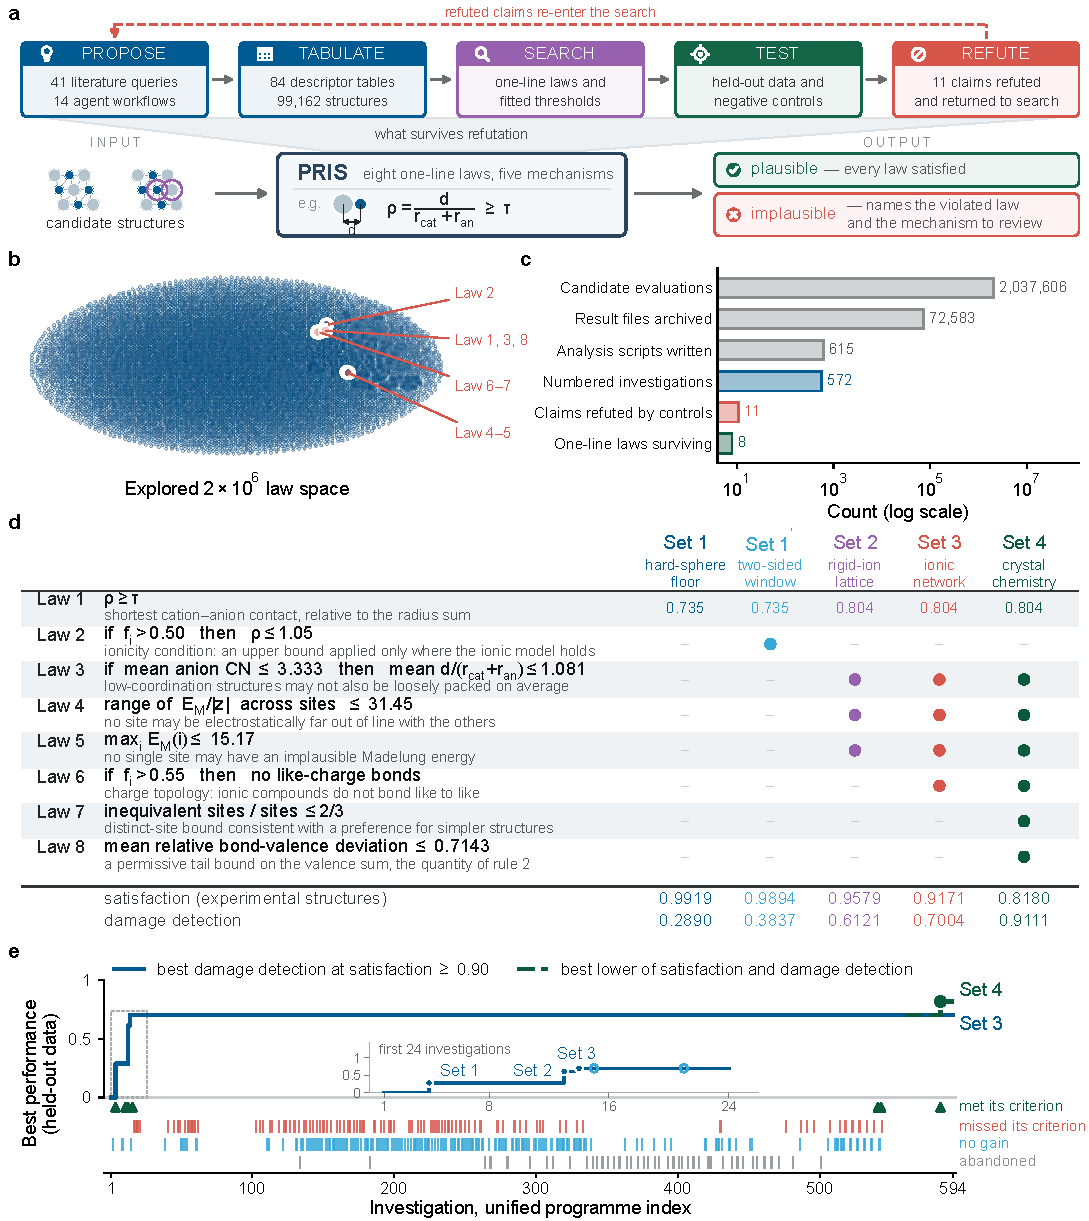
\includegraphics[width=0.99\textwidth]{figs/fig1_agentic_law_learning.pdf}
  \vspace{16pt}
  \caption{\textbf{Autonomous discovery by proposal, testing and refutation.}
  \textbf{a},~Pre-specified workflow: candidate-law proposal, descriptor tabulation,
  systematic search, held-out testing and attempted refutation. The dashed
  arrow returns refuted claims to the next cycle. Below, the eight surviving laws judge a
  candidate structure plausible or implausible. An implausible verdict
  names the unsatisfied law and the mechanism to review. Purple rings on the input
  structures mark an exchanged pair.
  \textbf{b},~t-distributed stochastic neighbour embedding (t-SNE) projection of the
  archived one-line candidate-law statements. Blue intensity encodes the number of
  statements per bin on a logarithmic scale. Red circles locate the statements nearest
  Law~1--Law~8.
  \textbf{c},~Counts of candidate evaluations, archived result files, analysis scripts,
  investigations, refuted claims and surviving laws (logarithmic axis).
  \textbf{d},~Law~1--Law~8, their predicates and their membership in the five nested sets,
  each named for the crystal model it enforces, with held-out satisfaction and damage detection for
  each set.
  \textbf{e},~Running best held-out performance versus investigation index: damage
  detection subject to the satisfaction floor (blue) and the smaller of satisfaction and
  detection (green). The inset enlarges the earliest investigations, and the strip beneath
  shows investigation outcomes.}
  \label{fig:loop}
\end{figure}

We drew fixed splits from 99{,}162 experimental ionic structures in the
ICSD and COD \cite{zagorac2019recent,grazulis2009crystallography} (details in Methods and Supplementary
Fig.~\ref{si-sifig:ranking-data}). We generated each damaged structure
from an experimental parent by a known displacement, strain or element exchange.
Across 572 investigations spanning plausibility, stability and synthesis, our agents
logged 2{,}037{,}606 candidate evaluations (Fig.~\ref{fig:loop}b,c). Every additional check
gave a passing claim another way to fail, and eleven initially successful conclusions
later failed these checks (Supplementary Section~\ref{si-note:s6}). The failures arose from misleading metrics
or class imbalance, laws recognising the perturbation procedure, and implementation errors.
The best law set improved only four times, the
last after more than five hundred investigations (Fig.~\ref{fig:loop}e). Eight one-line laws survived these two
million evaluations and now form PRIS.

The eight laws fall into nested sets, each demanding a fuller model of an ionic crystal
(Fig.~\ref{fig:loop}d): a hard-sphere contact floor (Set~1); the two-sided contact window in ionic
compounds (Set~1$'$); the rigid-ion lattice with packing and Madelung laws (Set~2); that
lattice as a charge-consistent bond network (Set~3); and full crystal chemistry with
valence and site laws (Set~4). Each set asks how much of the crystal a screen must model to
approach the achievable satisfaction--detection frontier (Fig.~\ref{fig:rules}a).
Supplementary Section~\ref{si-note:s18} gives definitions and domains.

\FloatBarrier
\subsection{Balancing experimental-structure satisfaction with damage detection}
\label{sec:rules}\label{sec:core}\label{sec:d1}\label{sec:d2}\label{sec:l4}

Satisfaction is the fraction of experimental structures that satisfy a law set under the
benchmark convention (details in Methods). Damage detection is the fraction of damaged structures
marked implausible by at least one law. A loose law that every structure satisfies scores
100\% satisfaction and 0\% detection. A strict law that rejects every structure scores
0\% satisfaction and 100\% detection. Both measurements are needed
(Fig.~\ref{fig:rules}a). Charge neutrality, a composition-only baseline, detected no
damage because every perturbation preserves composition. Fixed minimum-distance cutoffs, which are
element-blind, detected little damage.

Law~1 replaces the fixed distance with the radius-scaled reduced contact:
\begin{equation}
  \rhoc \equiv \min_{\mathrm{cation\text{--}anion\ contacts}}
  \frac{d}{r_{\mathrm{cat}}+r_{\mathrm{an}}},
  \label{eq:rho}
\end{equation}
where \(d\) is the contact distance and the denominator sums the Shannon radii
\cite{shannon1976revised}. A cutoff fixed in \AA{} is a larger fraction of the radius sum for a small ion pair, and
is therefore stricter for small ions. Set~1 requires \(\rhoc\geq0.735\), the first percentile
of the discovery distribution. It reached 99.2\% held-out satisfaction with 28.9\% damage
detection. If \rhoc{} is the coordinate that carries the physics, the energy cost of
compression should collapse onto it across chemistries. We rigidly scaled twenty experimental compounds
along \rhoc{}. In plane-wave DFT the cost crossed
0.1\,eV per atom at median \rhoc{} = 0.927. Both Law~1 floors lay inside a region already
costing electronvolts per atom, and the crossing was 1.80 times more tightly localised in
\rhoc{} than in \AA{} (Fig.~\ref{fig:anatomy}c).

Together, the eight laws are:
\begin{align*}
  \mathrm{Law\ 1}\quad & \rhoc \geq \tau,
    && \tau\in\{0.735,\,0.804\},\\
  \mathrm{Law\ 2}\quad & \fion>0.50 \ \Longrightarrow\ \rhoc\leq1.05,\\
  \mathrm{Law\ 3}\quad & \overline{\mathrm{CN}}_{\mathrm{an}}\leq3.333
    \ \Longrightarrow\
    \overline{d/(r_{\mathrm{cat}}+r_{\mathrm{an}})}\leq1.081,\\
  \mathrm{Law\ 4}\quad & \operatorname{range}_i\!\left(\VM(i)/v_i\right)\leq31.45\,\mathrm{eV},\\
  \mathrm{Law\ 5}\quad & \max_i \VM(i)\leq15.17\,\mathrm{eV},\\
  \mathrm{Law\ 6}\quad & \fion>0.55 \ \Longrightarrow\
    \text{no like-charge bonds},\\
  \mathrm{Law\ 7}\quad &
    n_{\mathrm{inequivalent\ sites}}/n_{\mathrm{sites}}\leq2/3,\\
  \mathrm{Law\ 8}\quad &
    \overline{\left|\mathrm{BV\ sum}-v_i\right|/v_i}\leq0.7143 .
\end{align*}
Here \fion{} is Pauling's composition-based ionic-character estimate. \(\VM(i)\) is the
site Madelung energy from an Ewald sum over formal charges. The quantity
\(v_i=|z_i|\) is the magnitude of site \(i\)'s formal charge \(z_i\). BV denotes the bond
valence used in the bond-valence sum.
Figure~\ref{fig:loop}d lists the laws in each set and their thresholds. A
structure not meeting a trigger condition satisfies that conditional law. A structure
lacking a required input in deployment receives no verdict rather than a pass (details in Methods).

A single contact floor encodes only the repulsive wall, but expansion lengthens rather than
shortens contacts, and a cation--anion exchange can leave every coordinate unchanged. Because
distinct failures can share the same closest distance, Set~2 judges the rigid-ion lattice,
and Set~3 the bond network. On held-out data Set~3 reached
91.7\% satisfaction and 70.0\% damage detection, above 55.2\% in every damage class.
Relative to Set~1, it detected nearly two and a half times as much damage. The cost was
rejecting one experimental structure in twelve rather than one in a hundred and twenty.
Set~4 trades satisfaction for detection by adding a permissive bond-valence-deviation law
and an empirical distinct-site-fraction law. It reached 81.8\% satisfaction and 91.1\%
overall detection, with at least 73.4\% in every class (Fig.~\ref{fig:rules}b and
Supplementary Figs.~\ref{si-sifig:perclass} and~\ref{si-sifig:amplitude}). Set~4 detected more by combining laws that target different failures, not by tightening one
cutoff.

Neither familiar criterion reaches this balance: the distance cutoff detects too little
damage, whereas Pauling's rules reject too many experimental structures. Among 5{,}297
held-out experimental structures, only 6.5\% of the charge-balanced ionic subset satisfied
rules 2--5 jointly \cite{pauling1929principles,george2020limited}
(Fig.~\ref{fig:rules}c). PRIS occupies the useful region between them because it reads chemistry, not because it
is uniformly stricter. Each law's mechanism or empirical hypothesis fixes the
measured quantity, the failing direction and the domain. Only the revisable threshold comes
from the population. Verdicts should therefore survive a change of population (Supplementary
Fig.~\ref{si-sifig:split-consistency}). Because split assignment used structure identifiers,
68.5\% of held-out experimental structures shared a reduced composition with discovery.
On compositions absent from discovery, frozen Set~4 still reached 82.7\%
experimental-structure satisfaction and 91.9\% damage detection
(Supplementary Fig.~\ref{si-sifig:pris-composition-holdout}).

\begin{figure}[!t]
  \centering
  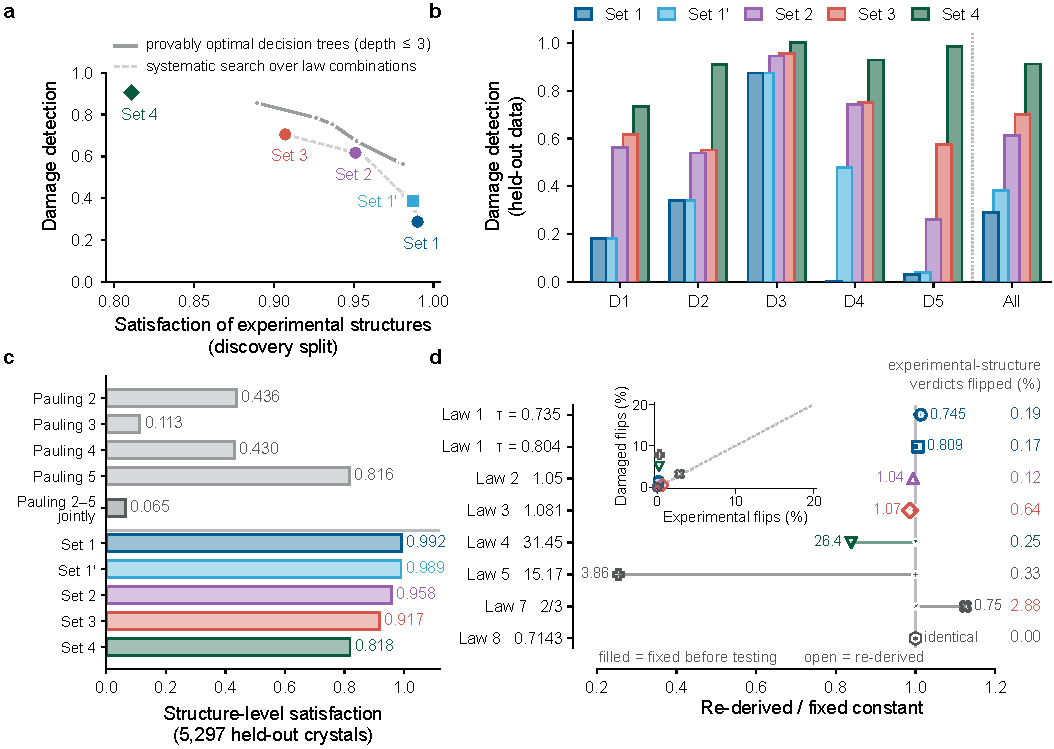
\includegraphics[width=\textwidth]{figs/fig2_rules.pdf}
  \caption{\textbf{Experimental-structure satisfaction, damage detection and threshold
  transfer.}
  \textbf{a},~Damage detection versus satisfaction on the discovery split: the
  depth-limited decision-tree frontier (solid grey), the systematic search over
  interpretable law combinations (dashed grey) and the five law sets (colours).
  \textbf{b},~Held-out damage detection by composition-preserving perturbation class and
  pooled (dotted divider).
  \textbf{c},~Satisfaction of Pauling rules 2--5, individually and jointly (grey), and of
  the five law sets (colours) on the same held-out structures.
  \textbf{d},~Law thresholds re-derived at their defining percentiles on held-out data,
  shown as the ratio to the frozen values, with unity meaning no change. The right-hand
  column gives the percentage of held-out experimental-structure verdicts that change.
  The inset compares verdict changes for experimental and chemically damaged structures on
  a common percentage scale, where the dashed line marks equality. Marker shape identifies
  the law in both the main panel and inset.}
  \label{fig:rules}
\end{figure}
\FloatBarrier

Thresholds shifted between the splits, but verdicts changed little. At the same held-out
percentiles, the contact, packing and bond-valence thresholds moved by at most 1.5\%. The two
electrostatic thresholds moved further (details in Methods). These larger shifts changed 5.0--7.8\% of verdicts on chemically damaged structures but only
0.25--0.33\% on experimental structures (inset, common 0--20\% scale).
Law~7 changed similar fractions in the two populations (3.2\% and 2.9\%, respectively;
Fig.~\ref{fig:rules}d). Separating mechanism from threshold keeps the laws testable rather than
reducing them to an opaque fitted score. Supplementary Figs.~\ref{si-sifig:threshold},
\ref{si-sifig:band-grid}, \ref{si-sifig:unguarded} and~\ref{si-sifig:chemistry} report
split transfer, threshold and band scans, and performance by anion family.

\subsection{From screening to diagnosis: five complementary mechanisms}
\label{sec:mechanism}

Structural implausibility arises through a few physical mechanisms, and each PRIS law is
written to test exactly one of them. Short-range repulsion (Law~1), ionic contact (Law~2)
and packing (Law~3) describe geometry. Electrostatic balance (Law~4--Law~6), bond-valence
conservation (Law~8) and crystallographic site complexity (Law~7) describe complementary
chemical and symmetry constraints without imposing a hierarchy. Figure~\ref{fig:anatomy}a shows their responses to five chemically damaged variants of
MgAl$_2$O$_4$, including an Mg--Al exchange that approximates natural inverse-spinel order.
Uniaxial compression lowers \rhoc{} from 0.99 to 0.76, whereas isotropic expansion raises it
to 1.28, beyond the 1.05 ceiling of Law~2. A
cation--anion exchange leaves \rhoc{} at 0.99 but creates eight like-charge bonds. No single
distance quantity captures all five mechanisms. Each unsatisfied law
names both the measured quantity and its mechanism.

\begin{figure}[tp]
  \centering
  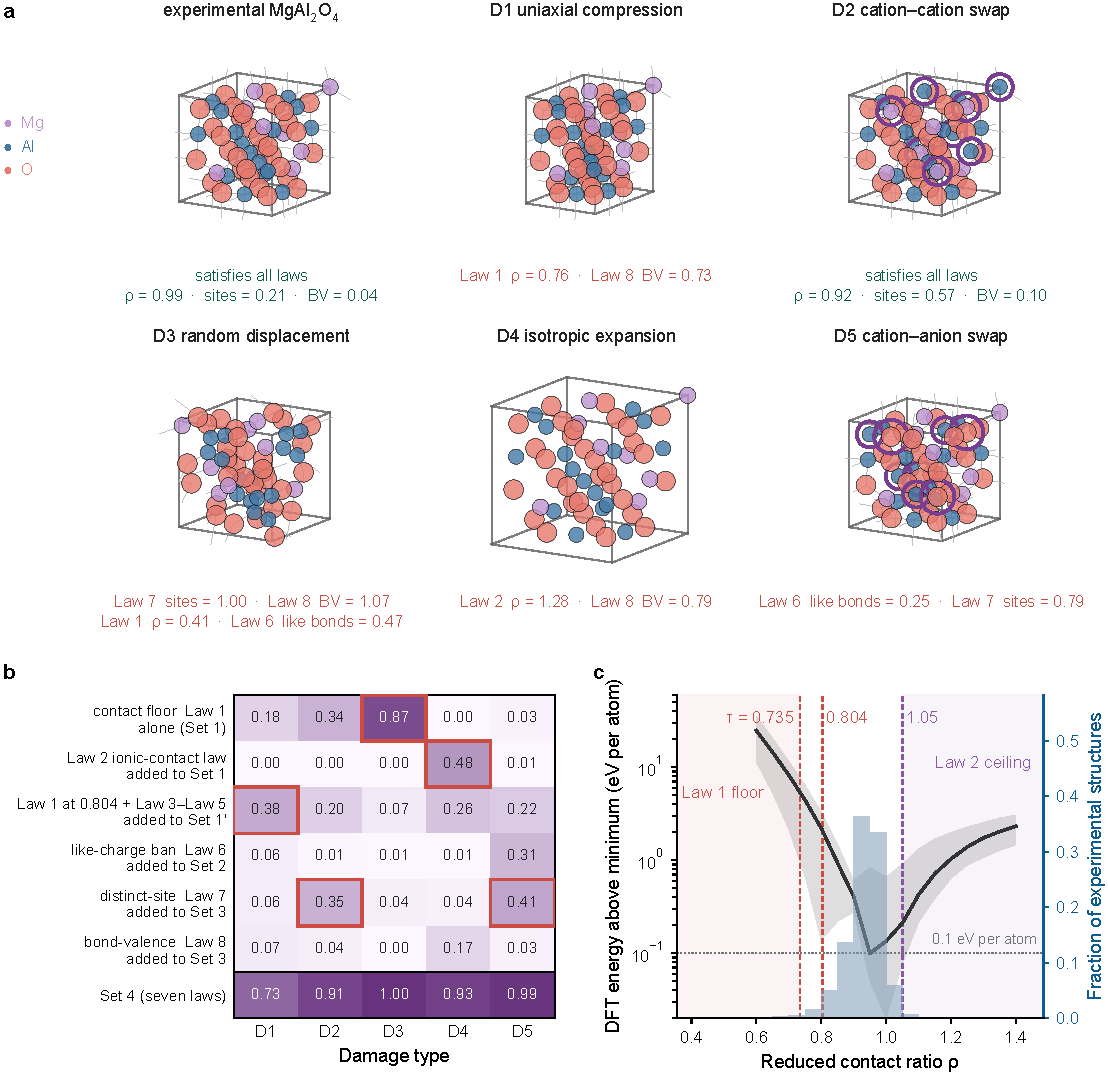
\includegraphics[width=\textwidth]{figs/fig3_anatomy.pdf}
  \caption[Physical basis of the laws]{\textbf{Physical basis of the PRIS plausibility
  laws.}
  \textbf{a},~Experimental MgAl$_2$O$_4$ and its five chemically damaged variants (uniaxial
  compression, cation--cation exchange, random displacement, isotropic expansion and
  cation--anion exchange), with the relevant descriptors and law verdicts beneath each
  structure (green satisfied, red unsatisfied); purple rings mark exchanged atoms.
  \textbf{b},~Held-out damage detection by perturbation class as laws are added,
  from Law~1 alone to Set~4; red outlines mark the combinations referenced in the text.
  \textbf{c},~DFT energy above each compound's own minimum for twenty experimental
  compounds rigidly scaled along the reduced-contact coordinate \rhoc{} (median and
  interquartile band, black, logarithmic left axis), together with the experimental
  distribution (blue, right axis). The two Law~1 floors and the conditional Law~2 ceiling
  are marked with their domains; the dotted line gives the pre-registered 0.1\,eV per atom
  cost. Per-compound curves, the hard-potential check and the spread of the crossing in
  each coordinate are in Supplementary Fig.~\ref{si-sifig:dft-e1-landscape}.}
  \label{fig:anatomy}
\end{figure}

The first mechanism, at the shortest length scale, is short-range repulsion, encoded by
Law~1. Coulomb attraction varies as \(1/d\), whereas closed-shell repulsion rises
approximately exponentially under compression \cite{born1932gittertheorie}, so a
sufficiently short ion pair is unlikely in an unconstrained local minimum
(Fig.~\ref{fig:anatomy}c). A floor cannot detect expansion, but in a
sufficiently ionic compound (\fion{} above 0.50) at least one cation--anion contact
should approach the radius sum \cite{hawthorne2026crystal}. Law~2 therefore marks a
shortest contact beyond 1.05 times that sum as unusually open. Within this domain, 96.25\% of
expanded discovery-split structures exceeded that ceiling, compared with 0.62\% of
experimental ionic structures. Law~3 limits packing differently: it caps the mean
reduced cation--anion contact at 1.081 when mean anion coordination is at most 3.333. Low coordination with long contacts indicates an open environment, so Law~3
detects expansion without Law~2's ionic-character requirement.

Geometry alone cannot detect a wrong-site exchange that changes no coordinate. Law~4--Law~6
instead look for three failures of electrostatic balance
\cite{ewald1921berechnung,hoppe1979effective}. Law~4 limits the range of site Madelung
energy divided by valence magnitude. Law~5 limits the largest site Madelung energy and catches a
single strongly destabilised site. For \fion{} above 0.55, Law~6 permits no like-charge
bond and therefore catches a cation--anion exchange that leaves the distance matrix
unchanged.
An Ewald sum does not test whether local bonds supply each ion's expected valence, but
Law~8 does. Bond valences decay exponentially with distance: expansion
lowers a site's sum, whereas compression or a wrong-site exchange can create an excess
\cite{brown2009recent,brese1991bond}. Across discovery and held-out structures with finite values,
the median of the mean relative deviation from nominal valence was 0.094 for experimental
structures and 0.705 for damaged ones.

The remaining mechanism counts distinct chemical environments. Under a stated symmetry
tolerance, Law~7 caps crystallographically inequivalent sites at two-thirds of all sites.
Moving atoms or reassigning elements often makes equivalent environments unique, whereas
experimental structures keep that fraction low. Law~7 thus turns Pauling's
preference for structural simplicity into an empirical chemical-order law. Each added
mechanism fills detection gaps that the earlier laws leave open in the held-out population
(Fig.~\ref{fig:anatomy}b). Together they turn screening into diagnosis by pointing the next
check at ionic size, oxidation state, site occupancy, local bonding or symmetry. Because these laws are physical rather than fitted, they should decide plausibility
before any relaxation is run.

\subsection{Screening candidates before expensive calculations}
\label{sec:certified}

Plausibility can be decided only from quantities an unrelaxed structure
already carries. In a validation queue, generators outpace the calculations that
relax and rank their output, so we benchmarked PRIS against
the 0.5- and 0.7-\AA{} cutoffs used in generator pipelines
\cite{xie2022crystal,betala2025lematgenbench} (details in Methods). These distance cutoffs detected only
1.6--3.2\% of the damage. On this benchmark, Set~4 reached 83.0\% satisfaction and detected
87.9\% of the damage (Fig.~\ref{fig:validation-synthesis}a). Set~4 still detected
2.6-fold more damage than a distance cutoff tightened to the same satisfaction (details in Methods).
An aggregate rate could be dominated by one easily detected perturbation, but
class-resolved rates ruled that out. Every mechanism detected the classes used to select it
and, more tellingly, classes withheld from that selection
\cite{geirhos2020shortcut,torralba2011unbiased,lapuschkin2019unmasking}
(Fig.~\ref{fig:validation-synthesis}b; details in Methods and Supplementary
Figs.~\ref{si-sifig:loko} and~\ref{si-sifig:validation-boundary-omission}a,b).

\label{sec:pauling}\label{sec:database}\label{sec:scores}\label{sec:formulas}

A plausible crystal must still be made, and ranking candidates by synthesizability requires a
continuous companion to the discrete PRIS laws. Our agents therefore fitted the
PRIS-derived synthesis score (PSS) on development pairs of recorded and computed-only
polymorphs with the same composition (details in Methods). The fitted score is
\begin{equation}
\begin{aligned}
  \mathrm{PSS}(\mathbf{x})={}&-4.90\,\widetilde v_{\mathrm{atom}}
  -1.24\,\widetilde M_z-1.18\,\widetilde\Delta_{\mathrm{BV}}
  -0.84\,\widetilde\eta_{\mathrm{site}} \\
  &-0.22\,\widetilde k_{\max}+0.59\,\widetilde f_{\mathrm{iso}},
  \qquad \widetilde x=\frac{x^\dagger-\mu_x}{\sigma_x}.
\end{aligned}
\label{eq:pss}
\end{equation}
The six terms, defined in Methods, are atomic volume, Madelung environment, bond-valence
deviation, distinct-site fraction, maximum cation-polyhedron connectivity and the fraction
of isolated cation polyhedra. The last two describe connectivity, and atomic volume has
the dominant negative coefficient, favouring density. Refitting on random halves of the
development structures reproduces the ranking and sign of every coefficient. The six terms
are correlated without being redundant (Supplementary
Figs.~\ref{si-sifig:pss-coefficient-stability} and~\ref{si-sifig:pss-term-correlation}). A
higher PSS marks a structure as easier to synthesize, and testing that
interpretation requires structures unlikely to be synthesized.

Labelled examples of such structures are scarce because databases record many successes
but few definitive failures. Positive--unlabelled (PU) learning estimates crystal likeness
through CLscore \cite{jang2020structure,song2025llm}. We trained two scorers on
experimental structures and an unlabelled LeMat and ELEMENTA pool
\cite{ramlaoui2025lemat,elementa2025dataset}. CGCNN-PU is a crystal
graph convolutional network with PU heads that learns its
representation within the synthesis task. The second model, MatterSim-1M-MLP-PU, instead freezes the representations of a universal
potential \cite{yang2024mattersim} and trains only the PU heads (details in Methods).
Agreement between these distinct routes reduces the risk of a model-specific artefact. The
364{,}592 unique structures ranked lowest by both machine-learning models are therefore
treated as the hard-to-synthesize cohort.

Set~4 and PSS answer different questions, and on the hard-to-synthesize cohort they
proved complementary. At 80.7\% experimental
satisfaction, Set~4 screened 51.9\% of this cohort, whereas PSS
screened 83.7\%
(Fig.~\ref{fig:validation-synthesis}c and Supplementary
Fig.~\ref{si-sifig:l4-contribution}a,b). A threshold on the MatterSim-computed energy above the convex hull,
\(E_{\mathrm{hull}}\), screened 72.0\% (details in Methods). Unlike PRIS and
PSS, however, this calculation requires relaxation and a phase hull. Because agreement
between the two models defines the hard-to-synthesize cohort, shared selection could create a CLscore trend
that neither model shows alone. We therefore tested the CLscore--Set~4 and CLscore--PSS
relations separately in each model.

Any relation with CLscore would be unexpected, because no synthesis label or PU output
entered the discovery of Law~1--Law~8. Both PU models gave the same directional relation
(details in Methods, Fig.~\ref{fig:validation-synthesis}d and Supplementary
Fig.~\ref{si-sifig:pu-model-performance}a--d). Across CLscore deciles, mean Set~4 violation
fell from 50.3\% to 30.4\% while mean PSS rose from $-11.37$ to $-0.18$. Linear fits of mean
PSS against decile index had $R^2=0.99$ for CGCNN-PU and $0.92$ for
MatterSim-1M-MLP-PU. Plausibility and predicted
synthesizability are linearly related across the population, but that link need not order
individual structures.

\begin{figure}[p]
  \centering
  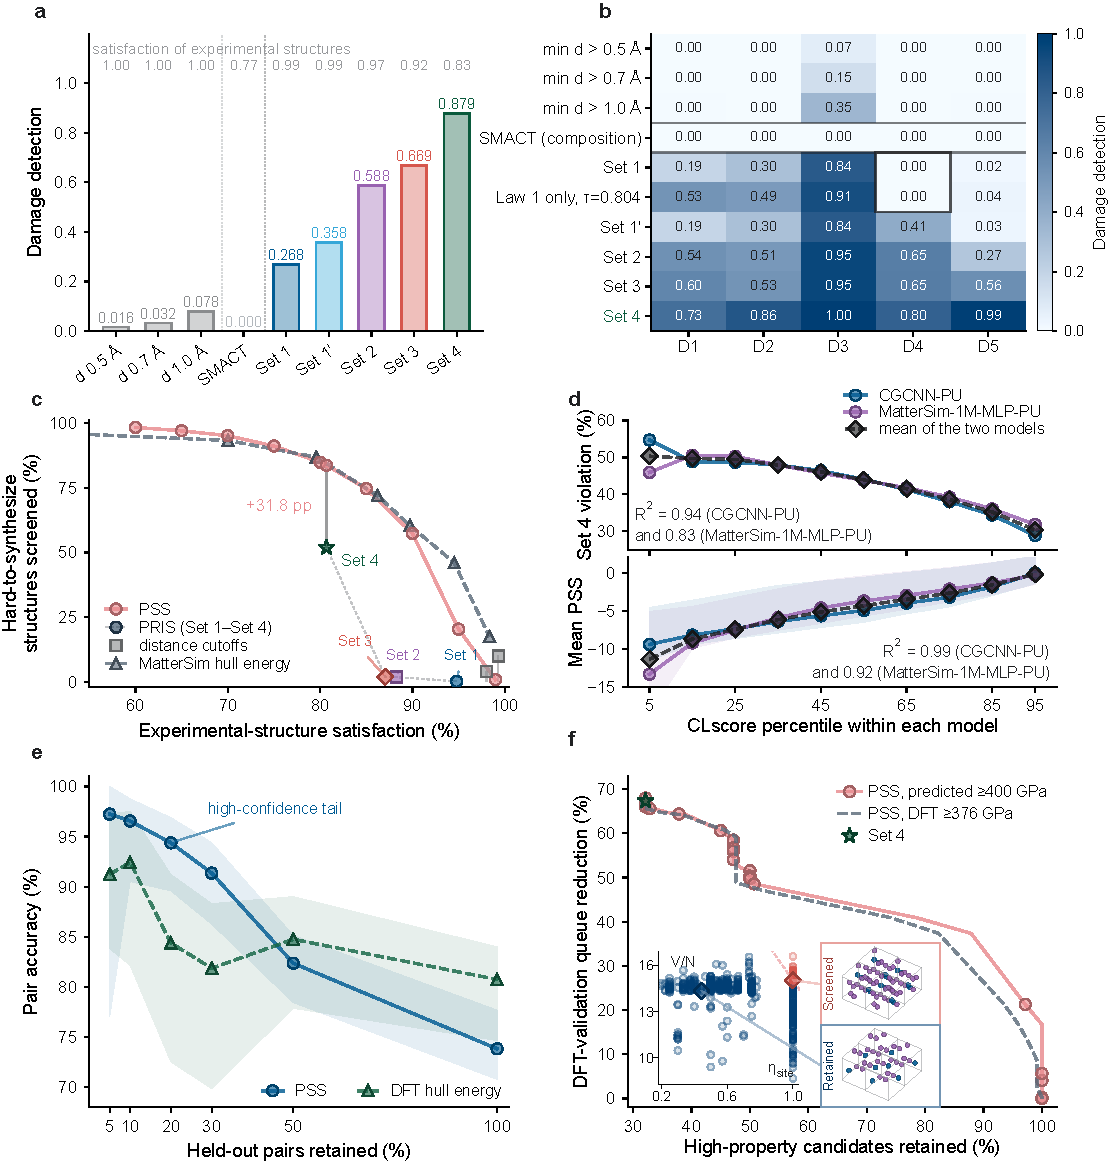
\includegraphics[width=\textwidth]{figs/fig4_validation_synthesis.pdf}
  \caption{\textbf{Physicochemical screening across validation tasks.}
  \textbf{a},~Overall damage detection for fixed-distance, composition-only and successive
  PRIS criteria; upper labels give satisfaction.
  \textbf{b},~Damage detection by perturbation class for baselines, contact laws and law
  sets. Outlines mark where a contact floor alone misses isotropic expansion.
  \textbf{c},~Satisfaction versus the fraction of hard-to-synthesize structures screened,
  for Set~1--Set~4, the PSS threshold sweep, distance cutoffs (grey squares) and a
  sweep over a MatterSim-computed hull-energy threshold (slate-grey triangles). Connectors
  join Set~4 and PSS at matched satisfaction.
  \textbf{d},~Set~4 violation and mean PSS across within-model CLscore deciles for
  CGCNN-PU, MatterSim-1M-MLP-PU and their pointwise mean. Shading spans each model's
  interquartile PSS range. Each panel gives the coefficient of determination for each
  model's straight-line fit against the decile index.
  \textbf{e},~Held-out same-composition pair accuracy for PSS and DFT
  \(E_{\mathrm{hull}}\) against the fraction of most-confident pairs retained (shading,
  confidence intervals).
  \textbf{f},~Across PSS thresholds, DFT-validation queue reduction versus retention of
  candidates that the universal machine-learned interatomic potential (UMA) predicts to
  have bulk modulus \(\geq400\)\,GPa; the Set~4 operating point is marked. The inset
  maps distinct-site fraction against atomic volume; blue and red points denote retained
  and screened candidates, respectively, and diamonds link a same-composition pair to the
  matching structure thumbnails. The dashed slate-grey curve uses the DFT-defined high-property
  subset at the mapped threshold of 376\,GPa among the 260 candidates evaluated from first
  principles (Supplementary Fig.~\ref{si-sifig:dft-e4-bulk}).}
  \label{fig:validation-synthesis}
\end{figure}

Plausibility asks whether a
structure could exist, whereas synthesis planning asks which credible polymorph to make
\cite{zeng2024selective}. Set~4 usually returned ties because several credible polymorphs
satisfy the same broad laws (details in Methods and Supplementary
Fig.~\ref{si-sifig:polymorph-ranking}a--c). Our own refutation step caught an error in the first
analysis: our agents had counted ties as ranking failures, making Pauling's rules appear
anti-predictive. Our agents then proposed a symmetry explanation, but auditing the same pairs within
composition refuted it. Treating ties as no decision removed the artefact.
The laws delimit a plausible region without ordering it. Within that region, PSS identified
the recorded polymorph in each pair with 68.1\% accuracy, compared with 75.0\% for DFT
\(E_{\mathrm{hull}}\) (details in Methods). On the most confident fifth of pairs, however, PSS reached 94.4\%
compared with 84.4\% for DFT (Fig.~\ref{fig:validation-synthesis}e). PSS can therefore place
high-confidence candidates first and leave the closer energy comparisons to DFT.

We conditioned independently seeded MatterGen runs on a bulk modulus of
400\,GPa. The runs yielded 1{,}081 unique, unrelaxed structures (details in Methods). UMA, a universal
machine-learned interatomic potential trained on no data from this work
\cite{wood2025uma}, predicted each candidate's bulk modulus and placed 140 of them at or
above the target. For the generated candidates, only the site-complexity and
atomic-volume terms of PSS were available. We therefore calibrated a PSS threshold on
experimental structures using those two terms (details in Methods). That threshold removed 61 candidates from the queue, but because the score is continuous, it is an operating point rather than a fixed rule. Across the threshold's range,
PRIS and PSS reduce the DFT validation queue by up to 67.3\%, and its setting
decides how many high-property candidates survive.

We checked those UMA predictions from first principles. At the median, DFT
bulk moduli for 260 candidates were 0.940 times the UMA predictions, so UMA predicted
higher values. The 400-GPa UMA target maps to 376\,GPa on the DFT
scale, and one candidate remained above 400\,GPa under DFT. Measured against that mapped
threshold, a high-property candidate outranked a removed
candidate 0.966 of the time, and 99.2\% of that high-property subset survived a screen that
cuts the queue by up to 67.3\%
(Fig.~\ref{fig:validation-synthesis}f and Supplementary
Fig.~\ref{si-sifig:dft-e4-bulk}).
Under DFT relaxation, sites that differ only in unconverged coordinates should merge, never
split further. On the generator's coordinates, 61
of the 260 candidates satisfied Law~7, and after DFT relaxation, 113 satisfied it. No candidate
moved in the opposite direction. Every additional Law~7 pass occurred among candidates
retained by PSS (Supplementary Fig.~\ref{si-sifig:dft-e4-composition}).

In the inset of Fig.~\ref{fig:validation-synthesis}f, the 61 PSS-screened candidates (red) all passed the
0.7-\AA{} cutoff but violated Law~7: every site was
crystallographically distinct at a 0.01-\AA{} tolerance. Their packing was also more open
than in the retained queue (details in Methods).

In a same-composition pair, the screened
Ir$_2$Os$_7$ candidate has P1 symmetry, 18 distinct sites among 18,
\(V/N=15.017\)\,\AA$^3$ and a PSS of $-0.638$. The retained candidate has C2/m symmetry,
four distinct sites among nine, \(V/N=14.327\)\,\AA$^3$ and a PSS of 1.245. Complete site
splitting with open packing again characterises the removed structures.
Because the discrete laws cannot weigh packing against site complexity, their operating
points fall at two extremes. Set~1--Set~3 retained all 140 high-property candidates but reduced
the queue by only 0--0.4\%. Set~4 reduced it by 67.3\% but lost most of those candidates
(details in Methods). Within the Set~4-violating subset, PSS screened structures that combined complete
site splitting with open packing. PSS retained 140 of 140 high-property candidates, including every one that Set~4 would
remove. These tunable PRIS and PSS operating points gave an
explainable reduction of the DFT validation queue by up to 67.3\%. PRIS
states why a structure is questionable, and PSS sets how strongly the queue is screened.

\subsection{Addressing controversy and identity failure in crystallography}
\label{sec:ordering-identity}

\label{sec:deploy}\label{sec:explain}

Beyond the queue, the same laws audit structures that have already been generated and
catalogued. Within every energy--phonon class, 84--89\% of recorded entries satisfied Law~7,
compared with 43--66\% of unrecorded entries (Supplementary
Fig.~\ref{si-sifig:energy-phonon-record}). A crystal can therefore pass distance cutoffs and
release little energy on relaxation while still splitting similar environments across too
many sites. Site ordering underlies both the proposed explanation for GNoME's low-symmetry
excess \cite{merchant2023scaling,cheetham2024artificial} and the A-Lab debate
\cite{szymanski2023autonomous,leeman2024challenges,szymanski2026correction,yamazaki2026navigating}.
Law~7 measures the excessive site splitting that geometric screens omit, so we tested it
first on public generators (Fig.~\ref{fig:deploy}).

\begin{figure}[!tp]
  \centering
  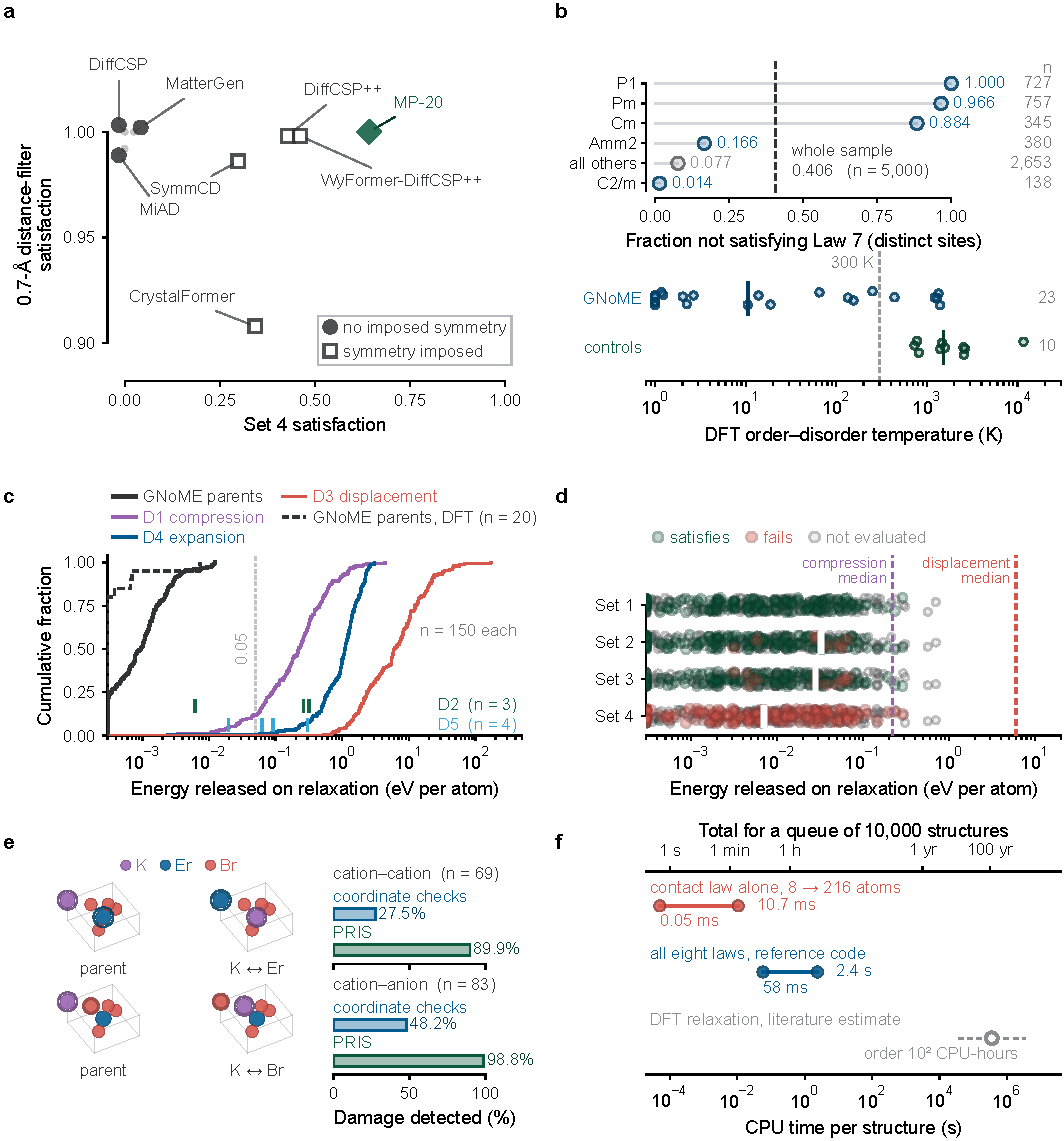
\includegraphics[width=0.975\textwidth]{figs/fig5_deployment.pdf}
  \caption{\textbf{Physicochemical screening of generated and database structures.}
  \textbf{a},~Minimum-distance-cutoff satisfaction versus Set~4 satisfaction among
  charge-assignable outputs from seven generators and from MP-20, the usual benchmark for
  these generators (green diamond). Filled circles mark generation without
  imposed symmetry, and open squares mark symmetry-constrained generation. Nearly
  coincident markers are offset and connected to their true coordinates.
  \textbf{b},~Upper, fraction of the GNoME sample failing Law~7 by source space group; the
  dashed line gives the whole-sample fraction. Lower, DFT order--disorder temperatures for
  23 label-merged GNoME entries and 10 experimental structures, obtained by relaxing every
  symmetry-distinct ordering of each entry. Vertical bars give class medians, and the dashed
  line marks 300\,K (Supplementary Fig.~\ref{si-sifig:dft-e2-ordering}).
  \textbf{c},~Cumulative distributions of the energy released on MatterSim relaxation for
  unmodified GNoME parents and their compressed, expanded and displaced counterparts.
  Sparse exchange classes appear as vertical marks. The dashed black curve gives the same
  quantity computed from first principles for twenty of these unmodified GNoME parents.
  Only the parents have a DFT curve because the DFT campaign's damaged cells come from
  experimental parents, a different population (Supplementary
  Fig.~\ref{si-sifig:dft-e3-paired}).
  \textbf{d},~Relaxation-energy release for raw MatterGen outputs resolved by Set~1--Set~4
  verdict. White vertical segments with pale-grey outlines mark failure-group medians; the
  two coloured dashed lines mark the compression and displacement medians of panel c. The energy axis keeps panel c's logarithmic
  decade spacing over a shorter range.
  \textbf{e},~Fixed-coordinate cation--cation and cation--anion exchanges in one
  KErBr$_4$ parent, with damage detection for four reimplemented coordinate checks
  and for the six PRIS laws on the same parent-matched exchanges.
  \textbf{f},~Measured CPU time per structure for Law~1 and for all eight laws, with the
  DFT-relaxation estimate from the literature (dashed). The upper axis converts the same
  values to total time for the displayed queue.}
  \label{fig:deploy}
\end{figure}

Avoiding overlap lets similar environments split. Placing atoms on
the Wyckoff positions of a chosen space group keeps them equivalent. We drew 500 unrelaxed structures from
each of seven public generators
\cite{zeni2025generative,jiao2023crystal,okhotin2025miad,jiao2024space,cao2025space,levy2025symmcd,kazeev2025wyckoff}.
The 0.7-\AA{} cutoff used in practice passed nearly all outputs and separated no model from
MP-20, the benchmark against which these generators are normally measured (details in Methods).
Set~4 instead exposed a pronounced dependence on imposed symmetry
(Fig.~\ref{fig:deploy}a). Among charge-assignable outputs, satisfaction was 0--2.5\%
without imposed symmetry, 29.9--46.1\% with it and 64.3\% for MP-20. Law~7 accounted for
much of this separation: generators failed it far more often than MP-20, even after
relaxation and symmetry analysis (details in Methods).
Every generator in the higher-satisfaction group builds its outputs on Wyckoff positions,
so the construction, not the sampler, decides how many outputs satisfy Set~4.

Law~7 needs no charge assignment, so it can audit a whole catalogue. We examined 5{,}000 uniformly drawn GNoME structures under a pre-fixed protocol
(details in Methods). Overall, 40.64\% failed Law~7, including all \(P1\) structures, with \(Pm\) and \(Cm\) structures failing nearly as often (Fig.~\ref{fig:deploy}b, upper; details in Methods; charge-law
coverage in Supplementary Fig.~\ref{si-sifig:charge-coverage}). Severe strain could mimic
this pattern, so we relaxed the same cells with MatterSim \cite{yang2024mattersim} to
measure the energy released by real damage. For the 150
unmodified GNoME parents, the median energy released on relaxation was less than
0.001\,eV per atom. Their compressed and displaced counterparts released
medians of 0.22 and 6.05\,eV per atom, respectively (Fig.~\ref{fig:deploy}c). To test whether this separation reflects the structures rather than the MatterSim potential, we recomputed 200 cells with DFT. MatterSim and DFT agreed, with a Spearman rank correlation of 0.953. Under DFT, twenty unmodified GNoME parents released a median of
0.0001\,eV per atom (dashed curve in Fig.~\ref{fig:deploy}c; Supplementary
Fig.~\ref{si-sifig:dft-e3-paired}).

Relaxation energy measures only the distance to a local minimum. Applied to 500 raw
MatterGen outputs grouped by their Set~4 verdict (details in Methods), it did not decide
plausibility. Failures released a median of 0.007\,eV per atom, close to
the 0.006\,eV per atom of the no-verdict group and far below both damage regimes
(Fig.~\ref{fig:deploy}d). Small relaxation energy therefore rules out gross strain but not
electrostatic, bond-valence or site-complexity failures. One chemical explanation remained untested: if artificial ordering creates the extra sites, merging similar species should restore equivalence.

We replaced chemically similar elements with one shared label. Of 150
sampled Law~7-failing entries, 113 contained a mergeable pair. At a symmetry tolerance of
0.1\,\AA{}, merging brought the distinct-site fraction to the Law~7 threshold or below in 78\% of
these entries. It raised the space-group symmetry in 79\%, a change that none of 27
mergeable experimental entries showed. Artificial ordering therefore explains much of the
sampled pattern and resolves the controversy for these entries: changing labels restores
equivalence without moving an atom.

An artificial ordering should cost nothing to permute. We relaxed with DFT every
symmetry-distinct ordering of 23 such entries and 10 experimental structures. Scrambling a
GNoME entry's ordering cost a median of 0.0001\,eV per atom, compared with 0.036\,eV per
atom for the experimental structures. The orderings became
interchangeable below 300\,K in 18 of the 23 GNoME entries and in none of the experimental
structures
(Fig.~\ref{fig:deploy}b, lower, and Supplementary
Fig.~\ref{si-sifig:dft-e2-ordering}). These energies put a number on the critique that generated catalogues substitute
nearly indistinguishable elements \cite{smit2026dataonly}.

The converse error leaves the geometry intact but assigns the wrong element to a fixed
site, and it has an experimental precedent. Harrison and colleagues reported at least 70
falsified structures in which genuine diffraction intensity data were reused after atomic
or metal identities were changed \cite{harrison2010falsified}. Hirshfeld rigid-bond alerts
and anomalous metal--ligand distances first exposed the problem, which structure-factor
comparisons then confirmed \cite{harrison2010falsified}. An element exchange at fixed coordinates redistributes formal charges, Madelung energies
and bond valences. Because those falsifications could also alter cell parameters and delete
reflections, we isolated chemical identity by exchanging species while holding the lattice
and every coordinate fixed.

On these parent-matched exchanges, we compared six PRIS laws (Law~1 and Law~4--Law~8)
with four reimplemented families of coordinate checks \cite{spek2009structure}
(Supplementary Section~\ref{si-note:s17}). The coordinate checks detected 19 of 69
cation--cation exchanges (27.5\%) and 40 of 83 cation--anion exchanges (48.2\%).
PRIS detected 62 of 69 cation--cation exchanges (89.9\%) and 82 of 83 cation--anion
exchanges (98.8\%; Fig.~\ref{fig:deploy}e). PRIS catches what the coordinate checks miss because electrostatics and bond valence
depend on chemical identity even when no atom moves.
The same mechanisms recur in a recovered archive of retracted depositions. Four evaluable
entries share one M(C$_2$H$_2$N$_3$Cl) framework, with M labelled Cu, Ni, Mn or Fe
\cite{iucr2012retraction}. The entries all gave \rhoc{} = 0.53 and mean bond-valence
deviations of 0.77--0.78, violating Law~1 and Law~8.

These diagnoses run on the structure as given, cheaply enough for routine use. Law~1
evaluates 10{,}000 cells of 6--20 atoms in under one second. All eight laws on the
same 10{,}000-cell queue take approximately ten minutes. The literature puts a DFT relaxation at 100\,CPU-hours, so the same queue
would cost approximately one million CPU-hours
(Fig.~\ref{fig:deploy}f) \cite{jain2013commentary}. A full PRIS evaluation therefore costs
under one millionth as much. Generators, structure-prediction workflows and autonomous
laboratories can run this screen before expensive validation, and each violation names the
mechanism to review.

What survives that screen still faces thermodynamic stability, dynamical stability and
synthesis, three assessments that do not track one another. On published phonon data
\cite{petretto2018highthroughput,zhu2024highthroughput}, 35.6\% of on-hull structures had
imaginary modes. Among recorded entries, 41.7\% were metastable. Conversely, 4{,}271
unrecorded entries were dynamically stable and within 50\,meV per atom of the hull (details in Methods).
None of these assessments asks whether the arrangement is physicochemically credible at all
\cite{sun2016thermodynamic,aykol2018thermodynamic,antoniuk2023predicting}, so plausibility
comes first rather than competing with them.

\section{Discussion}
\label{sec:ledger}

PRIS acts at three levels of decision: the validation queue, the database and the
individual site. At the queue level, population-derived conditional laws bridge the
restrictive Pauling rules and permissive distance cutoffs. A binary screen can legitimately
tie polymorphs within the plausible region, leaving PSS or energy to rank them. At the database
level, Law~7 and label merging both trace part of GNoME's low-symmetry excess to site
splitting by artificial ordering, the mechanism at issue in the ordering
controversy. At the site level, charge- and bond-valence-sensitive laws expose an incorrect
occupant at fixed coordinates. Coordinate-based screening cannot detect this failure.

Our discovery, benchmark and external tests establish structural plausibility as
an independent layer of assessment. This layer asks whether an arrangement obeys
physicochemical laws at all, so it precedes thermodynamic stability, dynamical
stability and synthesizability. These distinct questions cannot be collapsed into one
reconciling score, so the structural-plausibility check returns a falsifiable diagnosis instead.
Set~1--Set~4 demand a fuller model of the crystal as a task's risk rises. The
five mechanisms remain separate, with no imposed hierarchy, and every unsatisfied law names
the failure mechanism.

The five mechanisms also reach beyond plausibility. Laws discovered without synthesis labels
agree with two contrasting PU models, revealing an unexpected population-level link to
predicted synthesizability. PSS turns that link into a continuous, tunable score. In inverse
design, PSS weighs competing mechanisms: dense packing moderates a Law~7 warning, and the
structures PSS removes combine complete site splitting with open
packing. Together, PRIS and PSS link each anomaly to a measurable physical quantity
and remove chemically suspect candidates before expensive computation begins.
Beyond queue screening, the same verdicts can label database entries and training data. An
entry missing a charge or radius receives no verdict rather than a pass, keeping uncertain
entries separate from implausible ones.

Confidence in the structural-plausibility check rests on how the laws were retained. Active
refutation distinguished benchmark artefacts from real physics in an autonomous-agent
workflow \cite{boiko2023autonomous,szymanski2023autonomous,mbran2024augmenting}. Our agents
operated within goals and data boundaries set by humans. Across 572
investigations and 2{,}037{,}606 candidate evaluations, active refutation rejected eleven
initially successful conclusions and left eight compact laws. The preserved failure record
links each surviving law to the counterexamples and checks it withstood. Reporting
failed attempts has been called a condition for progress
\cite{smit2026dataonly}. This record is that report. Backed by the
record, crystal screening does not stop at a pass-or-fail verdict but explains why a
structure is implausible. Through active refutation, autonomous agents can discover
physicochemical laws that guide subsequent calculations and experiments.
